% =============================================================================
%              CHAPTER 3: MATERIALS AND METHODS
% =============================================================================
\chapter{Materials and Methods}

\section{Materials}

\subsection{Benchmark Datasets}

Two complementary action recognition datasets were selected to evaluate representation quality at different levels of semantic granularity: FineGym for fine-grained, visually similar action categories, and HMDB51 for coarse-grained, diverse human actions.

\subsubsection{FineGym}

FineGym \citep{shao2020finegym} is a large-scale, hierarchically annotated video dataset introduced at CVPR 2020 specifically designed to advance fine-grained action understanding in the domain of artistic gymnastics. FineGym organizes gymnastic routines into a three-level semantic hierarchy:

\begin{enumerate}[leftmargin=*]
    \item Event Level (Coarsest): Identifies the apparatus category---Balance Beam (BB), Floor Exercise (FX), Uneven Bars (UB), and Vault (VT).
    \item Set Level (Mid-level): Groups sub-actions into functionally related categories within each event (e.g., ``leap-jump-hop,'' ``beam-turns,'' ``dismount'').
    \item Element Level (Finest): Assigns specific, fine-grained labels to individual sub-actions (e.g., a particular type of double salto backward tucked). Standard benchmarking subsets at this level include Gym99 (99 element classes) and Gym288 (288 element classes).
\end{enumerate}

In this study, only the event-level annotations were used, treating the task as a 4-class classification problem. A balanced subset of 1,200 event clips (300 clips per apparatus category) was acquired from YouTube using \texttt{yt-dlp} with temporal trimming based on the official annotation timestamps. The event-level task was selected because it tests whether vision foundation models can distinguish between four apparatus routines that share substantial visual overlap---all featuring a single gymnast performing acrobatic movements in a competition arena---requiring the model to capture subtle differences in apparatus context, body orientation, and movement dynamics.

\subsubsection{HMDB51}

HMDB51 \citep{kuehne2011hmdb} is a widely adopted benchmark for general human action recognition, introduced at ICCV 2011 by the Serre Lab at Brown University. The dataset contains 6,766 video clips distributed across 51 action categories, with a minimum of 101 clips per class. Videos were primarily collected from digitized movies and public video repositories (YouTube, the Prelinger archive, and Google Videos), providing substantial diversity in viewpoint, background clutter, camera motion, lighting conditions, and video quality.

The 51 action classes span five broad categories of human motion:
\begin{enumerate}[leftmargin=*]
    \item General Facial Actions: e.g., smiling, laughing, chewing.
    \item Facial Actions with Object Manipulation: e.g., eating, drinking, smoking.
    \item General Body Movements: e.g., clapping, climbing, jumping, running.
    \item Body Movements with Object Interaction: e.g., brushing hair, catching, drawing sword, shooting a gun.
    \item Body Movements with Human Interaction: e.g., fencing, hugging, kicking, punching.
\end{enumerate}

HMDB51 serves as a complementary evaluation to FineGym: whereas FineGym tests fine-grained discrimination among visually similar classes, HMDB51 assesses the model's ability to handle a large number of semantically diverse action categories under challenging real-world conditions. The full dataset of 6,754 successfully loaded video clips (51 classes) was obtained as a 2.12~GB zip archive via the Hugging Face Hub (\texttt{jili5044/hmdb51}), with an 80/20 train/evaluation split applied during feature preprocessing.

\begin{table}[H]
\centering
\caption{Summary of evaluation datasets.}
\label{tab:dataset_summary}
\begin{tabular}{lrrcc}
\toprule
\textbf{Dataset} & \textbf{Clips} & \textbf{Classes} & \textbf{Task Granularity} & \textbf{Feature Dimension} \\
\midrule
FineGym & 1,200 & 4 & Fine-Grained & 1280 (V-JEPA 2.1) / 3584 (Qwen2.5-VL) \\
HMDB51  & 6,754 & 51 & Coarse-Grained & 1280 (V-JEPA 2.1) / 3584 (Qwen2.5-VL) \\
\bottomrule
\end{tabular}
\end{table}

\subsection{Vision Foundation Models}

Two vision foundation models representing fundamentally different representation learning paradigms were selected for comparative evaluation: V-JEPA~2.1 (self-supervised latent prediction) and Qwen2.5-VL (instruction-tuned vision-language model).

\subsubsection{V-JEPA~2.1 (Meta AI)}

V-JEPA~2.1 \citep{assran2025vjepa2, murlabadia2026vjepa21} is a 654-million parameter self-supervised video encoder based on the Vision Transformer Huge (ViT-H) architecture. Unlike generative models that reconstruct raw pixels, V-JEPA~2.1 learns representations by predicting masked spatiotemporal features in a learned latent space, entirely without language supervision or pixel reconstruction.

\paragraph{Spatiotemporal Tokenization.}
Input video clips are uniformly sampled to $T$ frames (8 frames in this study), each resized to $224 \times 224$ pixels. Frames are partitioned into non-overlapping spatiotemporal \emph{tubelets} of size $2 \times 16 \times 16$ (temporal $\times$ height $\times$ width) using a 3D convolutional patch embedding layer. Each tubelet is linearly projected to produce a $D$-dimensional token ($D = 1280$ for ViT-H), yielding a sequence of $N = \frac{T}{2} \times \frac{H}{16} \times \frac{W}{16}$ tokens per clip:
\begin{equation}
    \mathbf{z}_0 = \text{Conv3D}(\mathbf{V}) + \mathbf{E}_{\text{pos}}, \quad \mathbf{z}_0 \in \mathbb{R}^{N \times D}
    \label{eq:vjepa_tokenize}
\end{equation}
where $\mathbf{V} \in \mathbb{R}^{T \times H \times W \times 3}$ is the input video tensor and $\mathbf{E}_{\text{pos}}$ encodes positional information via 3D Rotary Position Embedding (RoPE), which injects explicit spatiotemporal coordinates into attention computations without fixed sinusoidal encodings.

\paragraph{Dual-Encoder Architecture.}
V-JEPA~2.1 employs a dual-encoder framework. Given two augmented views $x$ and $y$ of the same video clip, random spatiotemporal patches are masked from view $y$. The \emph{context encoder} $E_\theta$ (also called the x-Encoder) processes the full unmasked view $x$, while the \emph{target encoder} $E_{\bar{\theta}}$ (the y-Encoder) processes the complete view $y$ to produce target representations. The target encoder is not trained by gradient descent; instead, its weights $\bar{\theta}$ are updated as an Exponential Moving Average (EMA) of the context encoder weights:
\begin{equation}
    \bar{\theta} \leftarrow \tau \bar{\theta} + (1 - \tau) \theta, \quad \tau \in [0.996, 1.0)
    \label{eq:vjepa_ema}
\end{equation}

Both encoders are standard Vision Transformers consisting of $L$ layers of Multi-Head Self-Attention (MHSA) and Feed-Forward Network (FFN) blocks:
\begin{equation}
    \mathbf{z}'_l = \text{MHSA}(\text{LN}(\mathbf{z}_{l-1})) + \mathbf{z}_{l-1}, \quad
    \mathbf{z}_l = \text{FFN}(\text{LN}(\mathbf{z}'_l)) + \mathbf{z}'_l
    \label{eq:vjepa_transformer}
\end{equation}
where $\text{LN}(\cdot)$ denotes Layer Normalization and the attention mechanism uses Scaled Dot-Product Attention (SDPA) computed in float16 precision for memory efficiency.

\paragraph{Mask-Denoising Prediction Objective.}
A predictor network $P_\phi$, also parameterized as a Vision Transformer, takes the context encoder output $E_\theta(x)$ along with learnable mask tokens $\Delta_y$ (indicating the positions of dropped patches) and predicts the target representations of the masked regions. The V-JEPA~2.1 baseline training objective minimizes the $L_1$ distance between predicted and target representations:
\begin{equation}
    \underset{\theta,\,\phi,\,\Delta_y}{\text{minimize}} \quad \|P_\phi(\Delta_y, E_\theta(x)) - \operatorname{sg}(E_{\bar{\theta}}(y))\|_1
    \label{eq:vjepa2_obj}
\end{equation}
where $\operatorname{sg}(\cdot)$ is the stop-gradient operator that prevents representational collapse by blocking gradients through the target encoder. The loss is computed only over predictions corresponding to the masked patch positions.

\paragraph{Dense Per-Token Prediction Loss (V-JEPA~2.1).}
V-JEPA~2.1 \citep{murlabadia2026vjepa21} refines the training objective with a \emph{dense per-token prediction loss} that supervises each masked spatiotemporal token individually, rather than computing a single global loss:
\begin{equation}
    \mathcal{L}_{\text{predict}} = \frac{1}{|M|} \sum_{i \in M} \|P_\phi(E_\theta(x), \Delta_y)_i - \operatorname{sg}(E_{\bar{\theta}}(y)_i)\|_1
    \label{eq:vjepa21_obj}
\end{equation}
where $M$ is the set of masked patch indices and the subscript $i$ denotes the $i$-th token position. Additionally, a distance-weighted \emph{context loss} is applied to nearby visible tokens to enforce dense spatial grounding of context representations:
\begin{equation}
    \mathcal{L}_{\text{context}} = \frac{1}{|C|} \sum_{j \in C} \lambda_d(j) \cdot \|E_\theta(x)_j - \operatorname{sg}(E_{\bar{\theta}}(y)_j)\|_1
    \label{eq:vjepa21_context}
\end{equation}
where $C$ is the set of visible context token indices and $\lambda_d(j)$ is a distance-dependent weighting function that emphasizes tokens spatiotemporally proximate to masked regions. The total V-JEPA~2.1 objective combines both losses:
\begin{equation}
    \mathcal{L}_{\text{V-JEPA~2.1}} = \mathcal{L}_{\text{predict}} + \lambda_d \cdot \mathcal{L}_{\text{context}}
    \label{eq:vjepa21_total}
\end{equation}

\paragraph{Multi-Layer Intermediate Supervision.}
A critical innovation in V-JEPA~2.1 is the application of the prediction objective not only at the final encoder layer but at multiple intermediate depths. The predictor $P_\phi$ fuses features from selected encoder layers at approximately 25\%, 50\%, 75\%, and 100\% depth, ensuring that intermediate representations also acquire strong semantic features. This multi-layer supervision is directly exploited in the present study: features are extracted from these 4 intermediate layers with per-frame spatial mean pooling, producing a 4D tensor per clip:
\begin{equation}
    \mathbf{F}_{\text{multi}} = [\bar{\mathbf{z}}_{L/4};\; \bar{\mathbf{z}}_{L/2};\; \bar{\mathbf{z}}_{3L/4};\; \bar{\mathbf{z}}_{L}] \in \mathbb{R}^{4 \times T' \times D}
    \label{eq:vjepa_multilayer}
\end{equation}
where $\bar{\mathbf{z}}_l \in \mathbb{R}^{T' \times D}$ is the spatially mean-pooled representation at layer $l$ and $T'$ is the temporal token count after tubelet grouping. For baseline classifiers, the standard approach of global mean pooling over the final layer's output yields a single 1,280-dimensional embedding per clip: $\mathbf{f} = \frac{1}{N} \sum_{i=1}^{N} \mathbf{z}_{L,i} \in \mathbb{R}^{D}$.

\begin{figure}[H]
\centering
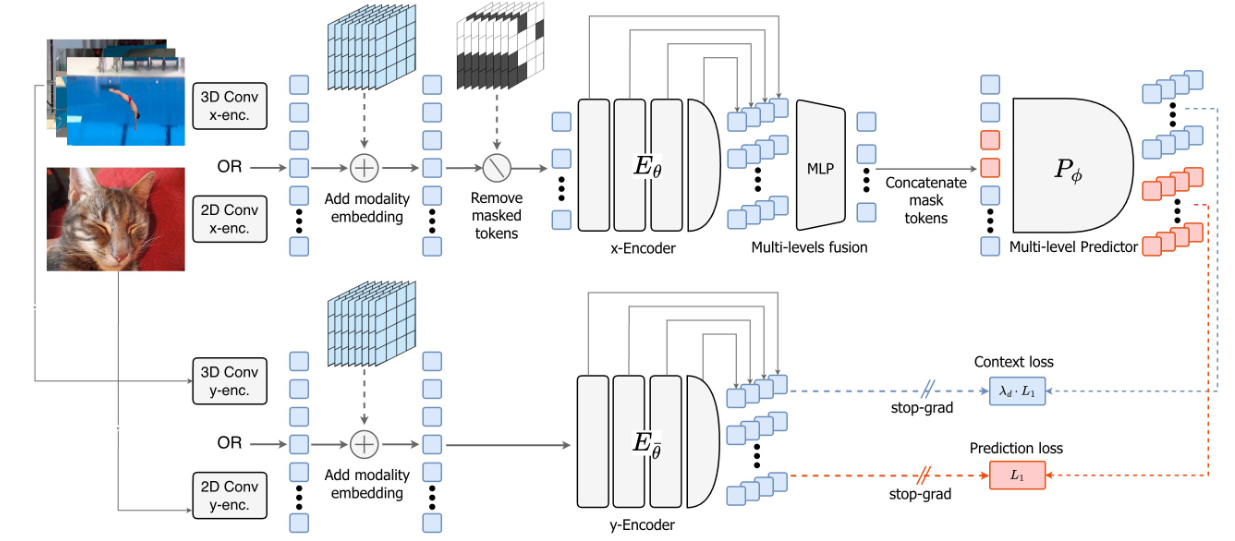
\includegraphics[width=\textwidth]{fig/vjepa2.png}
\caption{Architecture of V-JEPA~2.1 self-supervised pretraining framework showing the dual x-Encoder and y-Encoder pipeline with multi-level fusion, mask-denoising prediction, and stop-gradient targets \citep{murlabadia2026vjepa21}.}
\label{fig:vjepa2_arch}
\end{figure}

\subsubsection{Qwen2.5-VL (Alibaba Cloud)}

Qwen2.5-VL \citep{bai2025qwen2vl, qwen2025qwen3vl} is a 7-billion parameter autoregressive Vision-Language Model (VLM) that integrates visual understanding with language generation through cross-modal alignment. Unlike V-JEPA~2.1's purely visual self-supervised learning, Qwen2.5-VL acquires visual representations through joint training on massive image-text pairs and visual instruction tuning, producing features that are inherently grounded in linguistic semantics.

\paragraph{Vision Encoder and Native Dynamic Resolution.}
The Qwen2.5-VL Vision Encoder is a redesigned ViT trained from scratch to support \emph{native dynamic resolution} processing. Rather than resizing all inputs to a fixed resolution (e.g., $224 \times 224$), the encoder preserves the original aspect ratio and resolution of each input frame, partitioning it into non-overlapping patches of size $14 \times 14$ pixels. For video inputs, a 3D convolutional (Conv3D) patch embedding layer groups adjacent frames temporally (temporal stride of 2) to form spatiotemporal patches, reducing the total token count while preserving temporal context:
\begin{equation}
    \mathbf{v}_0 = \text{Conv3D}(\mathbf{V}_{\text{frames}}), \quad \mathbf{v}_0 \in \mathbb{R}^{N_v \times D_v}
    \label{eq:qwen_patchEmbed}
\end{equation}
where $N_v$ varies dynamically based on input resolution and $D_v$ is the vision encoder hidden dimension. This dynamic tokenization avoids information loss from aggressive resizing and produces a variable number of visual tokens per input.

\paragraph{Window Attention.}
To manage computational cost for high-resolution inputs, the Vision Encoder employs \emph{window attention} instead of global self-attention. Self-attention is computed locally within predefined spatial windows (e.g., $112 \times 112$ in patch space), reducing the computational complexity from $\mathcal{O}(N_v^2)$ to $\mathcal{O}(N_v \cdot w^2)$ where $w$ is the window size:
\begin{equation}
    \text{WindowAttn}(\mathbf{Q}, \mathbf{K}, \mathbf{V}) = \text{softmax}\!\left(\frac{\mathbf{Q}_w \mathbf{K}_w^T}{\sqrt{d_k}}\right) \mathbf{V}_w
    \label{eq:qwen_windowattn}
\end{equation}
where subscript $w$ denotes restriction to tokens within the same spatial window. This enables efficient processing of long video sequences without quadratic memory growth.

\paragraph{Multimodal Rotary Position Embedding (MRoPE).}
A key architectural innovation in Qwen2.5-VL is the \emph{Multimodal Rotary Position Embedding} (MRoPE), which extends the standard 1D RoPE used in language models to accommodate the multi-dimensional nature of visual inputs. The embedding dimension is decomposed into three segments, each encoding a separate positional axis---temporal ($t$), height ($h$), and width ($w$):
\begin{equation}
    \text{MRoPE}(\mathbf{x}, t, h, w) = \mathbf{x} \odot \left[\cos(\theta_t), \cos(\theta_h), \cos(\theta_w)\right] + \hat{\mathbf{x}} \odot \left[\sin(\theta_t), \sin(\theta_h), \sin(\theta_w)\right]
    \label{eq:qwen_mrope}
\end{equation}
where $\theta_t$, $\theta_h$, and $\theta_w$ are the rotation angles computed from the respective positional indices, and $\hat{\mathbf{x}}$ denotes the rotated complement of $\mathbf{x}$. For video inputs, the temporal position IDs are aligned with \emph{absolute time} rather than frame indices, enabling the model to learn the pace of events and perform temporal grounding at second-level precision. Notably, when all three positional indices are set equal ($t = h = w$), MRoPE reduces to standard 1D RoPE, ensuring compatibility with pure text decoding.

\paragraph{Visual-Language Fusion.}
After the Vision Encoder processes visual inputs, the resulting visual tokens are projected into the language model's embedding space through a multi-layer perceptron (MLP) merger:
\begin{equation}
    \mathbf{v}_{\text{lang}} = \text{MLP}_{\text{merge}}(\mathbf{v}_{\text{enc}}), \quad \mathbf{v}_{\text{lang}} \in \mathbb{R}^{N_v' \times D_{\text{LM}}}
    \label{eq:qwen_merge}
\end{equation}
where $D_{\text{LM}} = 3584$ is the hidden dimension of the Qwen2.5 language model decoder. The projected visual tokens are interleaved with text tokens to form a unified multimodal sequence, which is processed autoregressively by the Qwen2.5 LM Decoder. The model is trained to maximize the conditional log-likelihood of the next token:
\begin{equation}
    \mathcal{L}_{\text{LM}} = -\sum_{t=1}^{T_{\text{seq}}} \log p_\theta(x_t \mid x_{<t}, \mathbf{v}_{\text{lang}})
    \label{eq:qwen_lm_obj}
\end{equation}

\paragraph{4-bit NF4 Quantization.}
Due to GPU memory constraints (15.6~GB VRAM on the NVIDIA Tesla T4), Qwen2.5-VL is loaded in 4-bit NormalFloat (NF4) quantization with double quantization via the BitsAndBytes library. NF4 quantization maps full-precision weights $\mathbf{W} \in \mathbb{R}$ to a 4-bit data type optimized for normally distributed neural network weights:
\begin{equation}
    \mathbf{W}_{\text{NF4}} = \text{quantize}_{\text{NF4}}\!\left(\frac{\mathbf{W}}{s}\right) \cdot s, \quad s = \frac{\max(|\mathbf{W}_{\text{block}}|)}{q_{\max}}
    \label{eq:qwen_nf4}
\end{equation}
where $s$ is a per-block scaling factor and $q_{\max}$ is the maximum quantile value in the NF4 data type. Double quantization further compresses the scaling factors themselves to 8-bit, reducing the model memory footprint from approximately 14~GB (float16) to approximately 4~GB while preserving inference quality.

\paragraph{Feature Extraction Protocol.}
In this study, Qwen2.5-VL is used as a frozen feature extractor rather than a generative model. Four uniformly sampled frames per clip are processed through the Vision Encoder and LM Decoder via a minimal chat template prompt. The hidden states from the final decoder layer are mean-pooled across the sequence dimension to produce a single 3,584-dimensional embedding per clip:
\begin{equation}
    \mathbf{f}_{\text{Qwen}} = \frac{1}{T_{\text{seq}}} \sum_{t=1}^{T_{\text{seq}}} \mathbf{h}_t^{(L)}, \quad \mathbf{f}_{\text{Qwen}} \in \mathbb{R}^{3584}
    \label{eq:qwen_feat}
\end{equation}

\begin{figure}[H]
\centering
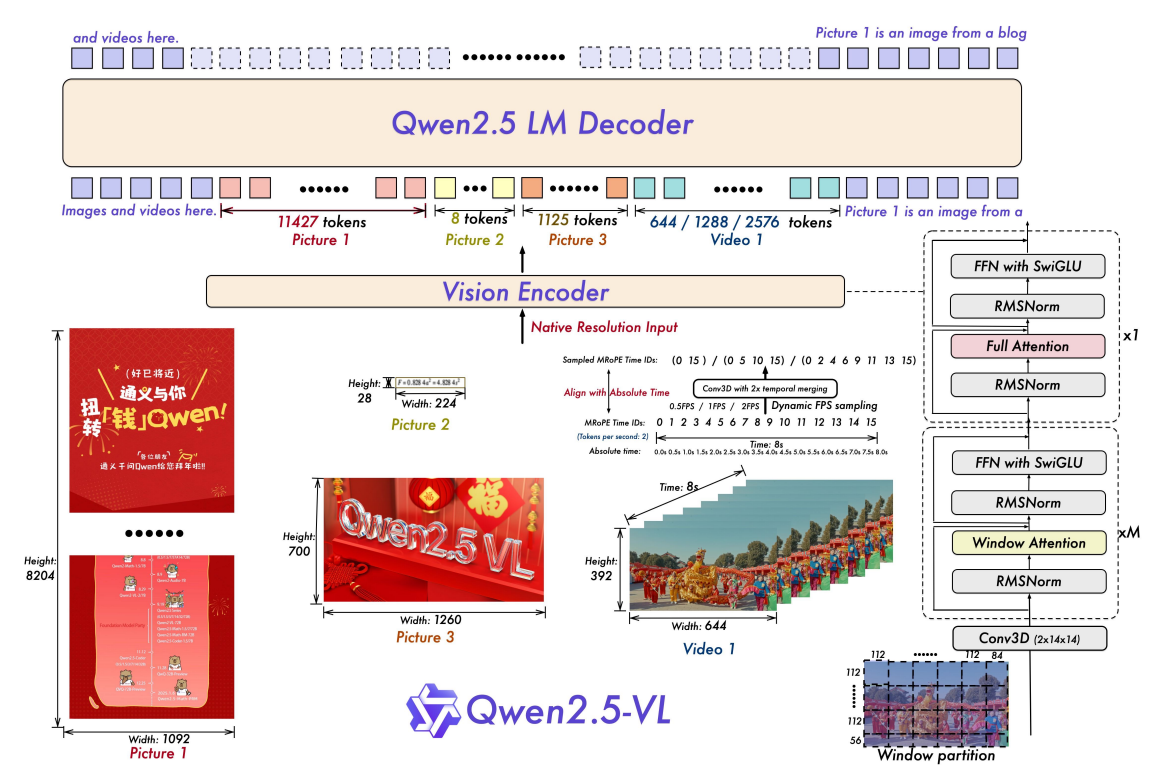
\includegraphics[width=\textwidth]{fig/qwen.png}
\caption{Architecture of Qwen2.5-VL vision-language model illustrating the Vision Encoder with Conv3D patch embedding, window attention, and native resolution input processing, feeding into the Qwen2.5 LM Decoder with MRoPE temporal alignment \citep{qwen2025qwen3vl}.}
\label{fig:qwen_arch}
\end{figure}


\section{Methods}

\subsection{Experimental Pipeline and Flowchart}

The experimental pipeline follows a structured sequence: video frame extraction, multi-layer feature vector extraction, standardization, dimensionality reduction via Principal Component Analysis (PCA), and multi-classifier evaluation including the novel HAF-STD Net architecture. Figure~\ref{fig:methodology_detailed} illustrates the pipeline.

\begin{figure}[p]
\centering
\vspace*{\fill}
\begin{tikzpicture}[
    node distance=0.8cm,
    block/.style={rectangle, draw, fill=blue!8, text width=4.2cm, text centered, rounded corners, minimum height=1.0cm, font=\normalsize},
    modelblock/.style={rectangle, draw=orange!70!black, fill=orange!12, text width=4.2cm, text centered, rounded corners, minimum height=1.8cm, font=\normalsize},
    procblock/.style={rectangle, draw=green!60!black, fill=green!8, text width=10.0cm, text centered, rounded corners, minimum height=1.0cm, font=\normalsize},
    pcablock/.style={rectangle, draw=green!60!black, fill=green!8, text width=10.0cm, text centered, rounded corners, minimum height=1.0cm, font=\normalsize},
    branchblock/.style={rectangle, draw=green!60!black, fill=green!8, text width=4.2cm, text centered, rounded corners, minimum height=1.4cm, font=\small},
    trainblock/.style={rectangle, draw=cyan!60!black, fill=cyan!10, text width=4.2cm, text centered, rounded corners, minimum height=1.4cm, font=\small},
    novelblock/.style={rectangle, draw=red!70!black, fill=red!8, text width=4.2cm, text centered, rounded corners, minimum height=1.4cm, font=\small},
    resultblock/.style={rectangle, draw=yellow!60!black, fill=yellow!12, text width=10.0cm, text centered, rounded corners, minimum height=1.0cm, font=\normalsize},
    arrow/.style={->, >=stealth, thick, line width=1pt},
    redarrow/.style={->, >=stealth, thick, line width=1.2pt, dashed, red!70!black},
]
    % === Stage 1: Data Sources ===
    \node[block] (fg_src) {\textbf{FineGym}\\1,200 clips\\4 event classes};
    \node[block, right=1.2cm of fg_src] (hmdb_src) {\textbf{HMDB51}\\6,754 clips\\51 action classes};

    % === Stage 2: Frame Extraction ===
    \node[procblock, below=1.0cm of $(fg_src.south)!0.5!(hmdb_src.south)$] (frames) {\textbf{Frame Extraction}\\OpenCV \texttt{VideoCapture} $\rightarrow$ Uniform temporal sampling $\rightarrow$ Resize to $224\times224$};

    % === Stage 3: Feature Extractors ===
    \node[modelblock, below left=1.2cm and 0.8cm of frames.south] (vjepa) {\textbf{V-JEPA~2.1}\\ViT-Huge, float16+SDPA\\8 frames $\rightarrow$ 4 layers\\$\times\;T'\!\times\!1280$};
    \node[modelblock, below right=1.2cm and 0.8cm of frames.south] (qwen) {\textbf{Qwen2.5-VL}\\4-bit NF4 quantized\\4 frames $\rightarrow$ 3584-d\\hidden-state pooling};

    % === Stage 4a: Feature Preprocessing — StandardScaler (all classifiers) ===
    \node[procblock, below=1.2cm of $(vjepa.south)!0.5!(qwen.south)$] (scaler) {\textbf{Feature Preprocessing}\\StandardScaler (zero mean, unit variance) $\rightarrow$ 80/20 Train/Eval Split};

    % === Stage 4b: PCA Dimensionality Reduction (baseline classifiers only) ===
    \node[pcablock, below=0.9cm of scaler] (pca) {\textbf{PCA Dimensionality Reduction}\\95\% variance retained $\rightarrow$ compact subspace ($k^* \ll D$)};

    % === Stage 5: Classifier Branches ===
    % HAF-STD Net (far left — multi-layer features, uses StandardScaler but bypasses PCA)
    \node[novelblock, below left=1.4cm and 3.5cm of pca.south] (hafstd) {\textbf{HAF-STD Net}\\{\scriptsize 4.8M params}};
    % Classical ML (center — shared path, both models)
    \node[branchblock, below=1.4cm of pca] (classify_sk) {\textbf{Classical ML (3)}\\SVM-RBF $\cdot$ Random Forest\\LogReg};
    % Neural Network Baselines (right — shared path, both models)
    \node[trainblock, below right=1.4cm and 3.5cm of pca.south] (classify_pt) {\textbf{Neural Network Classifiers (5)}\\MLP $\cdot$ DeepMLP $\cdot$ ResMLP\\Conv1DNet $\cdot$ Transformer};

    % === Stage 6: Comparative Evaluation ===
    \node[resultblock, below=1.4cm of classify_sk] (results) {\textbf{Comparative Evaluation}\\Accuracy, Macro/Weighted F1, MCC, Cohen's $\kappa$};

    % ====== ARROWS ======

    % Data sources -> Frame extraction
    \draw[arrow] (fg_src.south) -- (fg_src.south |- frames.north);
    \draw[arrow] (hmdb_src.south) -- (hmdb_src.south |- frames.north);

    % Frame extraction -> Models
    \draw[arrow] (frames.south -| vjepa.north) -- (vjepa.north);
    \draw[arrow] (frames.south -| qwen.north) -- (qwen.north);

    % Models -> StandardScaler (mean-pooled features for baselines, multi-layer for HAF-STD)
    \draw[arrow] (vjepa.south) -- (vjepa.south |- scaler.north)
        node[midway, right, font=\scriptsize\itshape, text=black!60] {Mean-pooled};
    \draw[arrow] (qwen.south) -- (qwen.south |- scaler.north);

    % V-JEPA multi-layer features -> StandardScaler (HAF-STD path enters preprocessing)
    \draw[redarrow] (vjepa.west) -- node[above, font=\scriptsize\itshape, text=red!70!black, align=center] {Multi-layer\\features} ++(-1.2, 0) |- (scaler.west);

    % StandardScaler -> PCA (baseline path)
    \draw[arrow] (scaler.south) -- (pca.north);

    % StandardScaler -> HAF-STD Net (bypasses PCA)
    \draw[redarrow] (scaler.south west) ++(0.3,0) -- ++(0,-.45) -| (hafstd.north);

    % PCA -> Shared classifier branches (two-way fan)
    \coordinate (fan) at ($(pca.south) + (0,-0.8)$);
    \draw[thick] (pca.south) -- (fan);
    \draw[arrow] (fan) -- (classify_sk.north);
    \coordinate (above_pt) at (fan -| classify_pt.north);
    \draw[thick] (fan) -- (above_pt);
    \draw[arrow] (above_pt) -- (classify_pt.north);

    % Shared classifiers -> Comparative Evaluation (fan-in)
    \coordinate (merge) at ($(classify_sk.south) + (0,-0.8)$);
    \draw[thick] (classify_sk.south) -- (merge);
    \draw[arrow] (merge) -- (results.north);
    \draw[arrow] (classify_pt.south) |- (merge);

    % HAF-STD -> Comparative Evaluation (dashed red path along left side)
    \draw[redarrow] (hafstd.south) |- (results.west);

\end{tikzpicture}
\vspace*{\fill}
\caption{Methodology flowchart showing the experimental pipeline.}
\label{fig:methodology_detailed}
\end{figure}

\clearpage
\subsection{Frozen-Feature Protocol}

Under the frozen-feature protocol \citep{assran2023ijepa, assran2025vjepa2}, backbone model weights $\mathbf{\Theta}$ remain fixed throughout downstream training:
\begin{equation}
\mathbf{z}_i = f(\mathbf{x}_i; \mathbf{\Theta}_{\text{frozen}}), \quad \nabla_{\mathbf{\Theta}} \mathcal{L} = \mathbf{0}
\end{equation}
Only downstream classifier weights $\mathbf{W}_{\text{head}}$ are optimized:
\begin{equation}
\mathbf{W}_{\text{head}}^* = \arg\min_{\mathbf{W}_{\text{head}}} \frac{1}{N}\sum_{i=1}^{N} \mathcal{L}\left( g(\mathbf{z}_i; \mathbf{W}_{\text{head}}), y_i \right)
\end{equation}

\subsection{Feature Preprocessing and PCA Dimensionality Reduction}

Extracted raw feature representations $\mathbf{Z} \in \mathbb{R}^{N \times D}$ are first standardized to zero mean and unit variance using the training-split statistics:
\begin{equation}
\tilde{\mathbf{z}}_{ij} = \frac{z_{ij} - \mu_j}{\sigma_j}, \quad \mu_j = \frac{1}{N_{\text{train}}} \sum_{i=1}^{N_{\text{train}}} z_{ij}, \quad \sigma_j = \sqrt{\frac{1}{N_{\text{train}}-1} \sum_{i=1}^{N_{\text{train}}} (z_{ij} - \mu_j)^2}
\label{eq:standardization}
\end{equation}
where $j \in \{1, \ldots, D\}$ indexes feature dimensions. Standardization ensures that all features contribute equally to the subsequent dimensionality reduction step, preventing high-variance dimensions from dominating the principal component decomposition. The same $\mu_j$ and $\sigma_j$ statistics computed from the training split are applied to the test split to avoid data leakage.

Principal Component Analysis (PCA) is then applied to project the standardized features into a lower-dimensional, decorrelated subspace. Given the standardized feature matrix $\tilde{\mathbf{Z}} \in \mathbb{R}^{N \times D}$, PCA computes the covariance matrix:
\begin{equation}
\mathbf{C} = \frac{1}{N_{\text{train}}-1} \tilde{\mathbf{Z}}_{\text{train}}^\top \tilde{\mathbf{Z}}_{\text{train}} \in \mathbb{R}^{D \times D}
\label{eq:covariance}
\end{equation}
and performs eigendecomposition $\mathbf{C} = \mathbf{V} \boldsymbol{\Lambda} \mathbf{V}^\top$, where $\boldsymbol{\Lambda} = \text{diag}(\lambda_1, \lambda_2, \ldots, \lambda_D)$ contains eigenvalues sorted in descending order ($\lambda_1 \ge \lambda_2 \ge \cdots \ge \lambda_D \ge 0$) and $\mathbf{V} = [\mathbf{v}_1, \mathbf{v}_2, \ldots, \mathbf{v}_D]$ contains the corresponding orthonormal eigenvectors (principal components). The number of retained components $k^*$ is selected as the minimum $k$ that preserves at least 95\% of the total variance:
\begin{equation}
k^* = \arg\min_{k} \left( \frac{\sum_{j=1}^{k} \lambda_j}{\sum_{j=1}^{D} \lambda_j} \ge 0.95 \right)
\label{eq:pca_k}
\end{equation}
The projection onto the retained subspace is then given by:
\begin{equation}
\mathbf{Z}_{\text{PCA}} = \tilde{\mathbf{Z}} \, \mathbf{V}_{:k^*} \in \mathbb{R}^{N \times k^*}
\label{eq:pca_projection}
\end{equation}
where $\mathbf{V}_{:k^*} \in \mathbb{R}^{D \times k^*}$ contains the first $k^*$ principal components.

The 95\% variance retention threshold was chosen as a standard balance between information preservation and dimensionality reduction. On the FineGym dataset, PCA reduced V-JEPA~2.1 features from $D=1{,}280$ to $k^*=90$ dimensions and Qwen2.5-VL features from $D=3{,}584$ to $k^*=142$ dimensions. On HMDB51, V-JEPA~2.1 features were reduced to $k^*=286$ and Qwen2.5-VL features to $k^*=719$ dimensions. The substantially higher retained dimensionality for HMDB51 reflects the greater representational complexity required to distinguish 51 action classes compared to FineGym's 4 classes.

PCA serves three key purposes in this pipeline: (1)~it decorrelates features, removing redundant collinear dimensions that arise from the over-parameterized encoder architectures; (2)~it reduces computational cost for the classical ML classifiers (SVM-RBF, Random Forest), which scale poorly with high-dimensional inputs; and (3)~it mitigates the curse of dimensionality, particularly for the smaller FineGym dataset where the sample-to-feature ratio would otherwise be unfavourable. Importantly, PCA is applied \textit{only} to the baseline classifier pathway. The HAF-STD Net receives the full-dimensional, multi-layer temporal tensor without PCA reduction, as its spectral-temporal decomposition module (Section~\ref{sec:hafstd_net}) operates directly on the spatiotemporal structure and benefits from preserving the complete representational capacity.


\subsection{Classifier Architectures}

Extracted features are evaluated across 8 baseline classifiers plus the HAF-STD Net architecture (9 classifiers total):

\subsubsection{Classical Machine Learning Classifiers}

\begin{enumerate}[leftmargin=*]
    \item \textbf{Support Vector Machine (SVM-RBF)} \citep{cortes1995svm}\textbf{:} Radial Basis Function kernel $K(\mathbf{x}_i, \mathbf{x}_j) = \exp\left(-\gamma \|\mathbf{x}_i - \mathbf{x}_j\|^2\right)$ with $C=1.0$.
    \item \textbf{Random Forest} \citep{breiman2001randomforests}\textbf{:} Ensemble of 500 decision trees with balanced class weighting.
    \item \textbf{Logistic Regression} \citep{cox1958logistic}\textbf{:} Linear probe with L2 regularization ($C=1.0$) and multinomial softmax.
\end{enumerate}

\subsubsection{Neural Network Classifiers}

\begin{enumerate}[leftmargin=*]
    \item \textbf{Multi-Layer Perceptron (MLP)} \citep{rumelhart1986backprop}\textbf{:} Scikit-learn MLP with 2 hidden layers (512, 256), ReLU, and Adam optimizer.
    \item \textbf{DeepMLP:} 4-layer feedforward network (Input $\rightarrow$ 512 $\rightarrow$ 256 $\rightarrow$ 128 $\rightarrow$ Classes) with BatchNorm \citep{ioffe2015batchnorm}, ReLU, and Dropout \citep{srivastava2014dropout} (0.3).
    \item \textbf{ResMLP} \citep{he2016resnet}\textbf{:} Deep residual MLP with skip connections: $\mathbf{h}_{l+1} = \mathbf{h}_l + \mathcal{F}(\mathbf{h}_l, \mathbf{W}_l)$.
    \item \textbf{Conv1DNet} \citep{lecun1998cnn}\textbf{:} 1D Convolutional network projecting feature dimension as spatial channels followed by adaptive max pooling.
    \item \textbf{MiniTransformer} \citep{vaswani2017attention}\textbf{:} Self-Attention transformer encoder block with multi-head attention ($h=4$) and feedforward projection.
\end{enumerate}

\subsubsection{HAF-STD Net Classifier}
\label{sec:hafstd_net}

We propose \textbf{HAF-STD Net} (Hierarchical Adaptive Fusion with Spectral-Temporal Decomposition), a specialized classification architecture that jointly exploits V-JEPA~2.1's unique properties of temporal coherence and deep self-supervision. The architecture contains 4.8M trainable parameters and operates on multi-layer per-frame features extracted from the frozen V-JEPA~2.1 encoder. HAF-STD Net introduces three core components:

\paragraph{1. Spectral-Temporal Decomposition via Haar DWT.}
A 1D Haar Discrete Wavelet Transform is applied along the temporal axis of V-JEPA~2.1's latent token sequences at each selected encoder layer. This decomposes the temporal signal into low-frequency (appearance/trend) and high-frequency (motion/change dynamics) components:
\begin{equation}
\mathbf{a}_k = \frac{1}{2}(\mathbf{h}_{2t} + \mathbf{h}_{2t+1}), \quad
\mathbf{d}_k = \frac{1}{2}(\mathbf{h}_{2t} - \mathbf{h}_{2t+1})
\end{equation}
where $\mathbf{a}_k$ captures static appearance and $\mathbf{d}_k$ captures motion dynamics at layer $k$. The mean-pooled approximation and detail coefficients form the \emph{appearance stream} and \emph{motion stream}, respectively.

\paragraph{2. Depth Representation Velocity.}
Inter-layer deltas are computed between consecutive selected encoder layers:
\begin{equation}
\Delta\mathbf{H}_k = \bar{\mathbf{H}}_{k+1} - \bar{\mathbf{H}}_k, \quad k \in \{1, 2, 3\}
\end{equation}
where $\bar{\mathbf{H}}_k$ denotes the temporally mean-pooled hidden state at layer $k$. These \emph{velocity vectors} capture how the model's internal understanding progressively transforms across its depth---a signal that is action-class-dependent due to V-JEPA~2.1's deep self-supervision training. Between the 4 selected layers, there are exactly $4 - 1 = 3$ consecutive inter-layer velocity vectors.

\paragraph{3. Adaptive Routing over Depth $\times$ Frequency Streams.}
The decomposed streams across layers (4 appearance streams, 4 motion streams, and 3 depth velocity streams) are independently projected through dedicated linear heads, yielding $4 + 4 + 3 = 11$ feature vectors. An adaptive routing network learns input-dependent fusion weights:
\begin{equation}
\mathbf{w} = \text{softmax}\left(\text{MLP}\left([\mathbf{s}_1; \mathbf{s}_2; \ldots; \mathbf{s}_{11}]\right)\right), \quad
\mathbf{f} = \sum_{i=1}^{11} w_i \cdot \mathbf{s}_i
\end{equation}
The fused representation $\mathbf{f}$ is classified via a cosine similarity head with learnable temperature scaling $\tau$:
\begin{equation}
p(y=c | \mathbf{f}) = \frac{\exp\left(\tau \cdot \hat{\mathbf{f}}^T \hat{\mathbf{w}}_c\right)}{\sum_{j=1}^{C} \exp\left(\tau \cdot \hat{\mathbf{f}}^T \hat{\mathbf{w}}_j\right)}
\end{equation}

\begin{figure}[H]
\centering
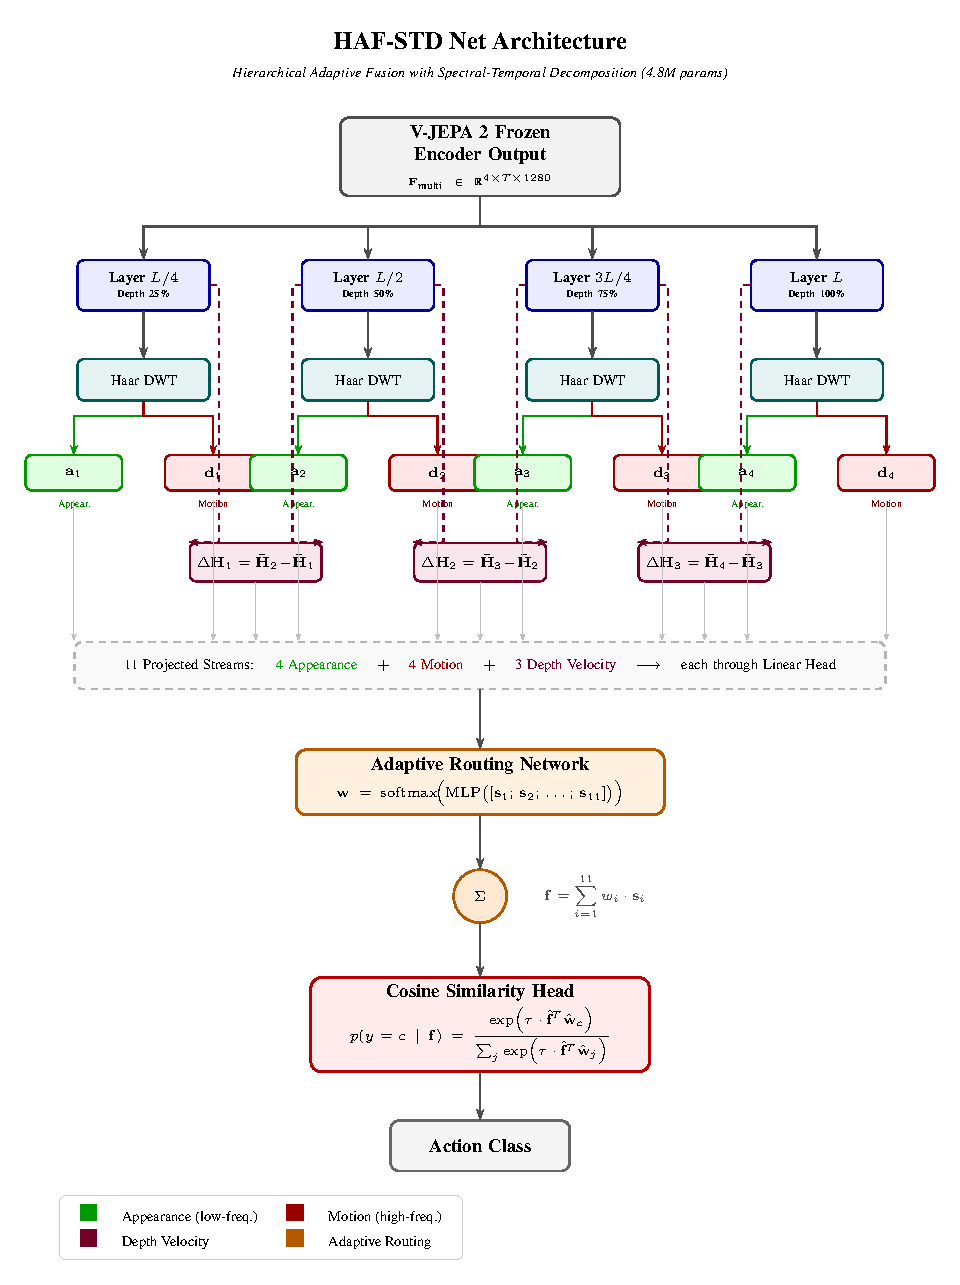
\includegraphics[width=\textwidth]{fig/hafstd_figure.pdf}
\caption{Architecture of the proposed HAF-STD Net classifier.}
\label{fig:hafstd_arch}
\end{figure}

\subsection{Training Techniques and Optimization}

All neural network classifiers are trained using:
\begin{itemize}[leftmargin=*]
    \item \textbf{Label Smoothing ($\epsilon = 0.1$):} Softens one-hot target vectors $y_c^{\text{smooth}} = (1 - \epsilon) y_c + \frac{\epsilon}{C}$.
    \item \textbf{Feature-Space Mixup ($\alpha = 0.2$):} Interpolates feature pairs: $\tilde{\mathbf{z}} = \lambda \mathbf{z}_i + (1-\lambda)\mathbf{z}_j$.
    \item \textbf{Cosine Annealing LR:} Learning rate schedule decaying from $10^{-3}$ to $10^{-6}$.
    \item \textbf{Optimizer:} AdamW with weight decay $\lambda=10^{-4}$.
    \item \textbf{Early Stopping:} Triggers after 15 epochs without validation loss improvement.
\end{itemize}

\subsection{Evaluation Metrics}
\label{sec:eval_metrics}

To thoroughly assess classification performance and mitigate potential biases arising from class imbalance or superficial prediction heuristics, model evaluation is grounded on a comprehensive suite of quantitative metrics. In this study, experiments encompass both fine-grained action classification on FineGym ($C = 4$ sub-action categories) and coarse-grained classification across diverse motion categories on HMDB51 ($C = 51$ classes).

\subsubsection{Confusion Matrix and Multi-Class Decomposition}

All evaluated metrics are derived from the empirical confusion matrix $\mathbf{M} \in \mathbb{N}^{C \times C}$, where each element $M_{ij}$ denotes the count of test samples whose true ground-truth class is $i$ but were classified into class $j$ by the model. The total number of evaluation samples is given by $N = \sum_{i=1}^{C}\sum_{j=1}^{C} M_{ij}$.

For any individual target class $c \in \{1, 2, \dots, C\}$, multi-class evaluation can be decomposed into a set of binary One-vs-Rest (OvR) classification problems using four fundamental quantities:
\begin{itemize}[leftmargin=*]
    \item \textbf{True Positives ($TP_c$):} The number of video instances correctly predicted as class $c$:
    \begin{equation}
    TP_c = M_{cc}
    \end{equation}
    \item \textbf{False Positives ($FP_c$):} The number of video instances belonging to classes other than $c$ that are incorrectly predicted as class $c$ (Type I error / false alarm):
    \begin{equation}
    FP_c = \sum_{i \neq c} M_{ic}
    \end{equation}
    \item \textbf{False Negatives ($FN_c$):} The number of video instances belonging to true class $c$ that are incorrectly assigned to a different class (Type II error / missed detection):
    \begin{equation}
    FN_c = \sum_{j \neq c} M_{cj}
    \end{equation}
    \item \textbf{True Negatives ($TN_c$):} The number of video instances not belonging to class $c$ that are correctly predicted as non-$c$:
    \begin{equation}
    TN_c = \sum_{i \neq c} \sum_{j \neq c} M_{ij} = N - TP_c - FP_c - FN_c
    \end{equation}
\end{itemize}
The total ground-truth support (number of true instances) for class $c$ is defined as $N_c = TP_c + FN_c = \sum_{j=1}^C M_{cj}$, while the total number of predictions assigned to class $c$ is $P_c = TP_c + FP_c = \sum_{i=1}^C M_{ic}$.

\subsubsection{Classification Accuracy}

Overall classification accuracy measures the fraction of all test video clips whose top predicted class label coincides with the ground-truth annotation:
\begin{equation}
\text{Accuracy} = \frac{\sum_{c=1}^{C} M_{cc}}{N} = \frac{1}{N}\sum_{i=1}^{N} \mathbf{1}\left(\hat{y}_i = y_i\right)
\end{equation}
where $\hat{y}_i = \arg\max_c \, p(y=c \mid \mathbf{x}_i)$ is the model's highest-probability predicted class for sample $\mathbf{x}_i$, $y_i$ is the corresponding ground-truth label, and $\mathbf{1}(\cdot)$ is the indicator function. 

In single-label multi-class video classification, this is standard overall accuracy (top-1 decision rule). Under uniform random chance, the expected accuracy corresponds to $1/C$, yielding $25.0\%$ for FineGym ($C = 4$) and approximately $1.96\%$ for HMDB51 ($C = 51$). While overall accuracy provides an intuitive global benchmark of model correctness, it weights all instances equally and can thus be dominated by high-support majority classes. Consequently, additional class-balanced and chance-adjusted metrics are required.

\subsubsection{Precision (Macro and Weighted)}

Precision assesses the reliability or purity of model predictions for a given category. For class $c$, it represents the probability that a sample predicted to be class $c$ truly belongs to class $c$:
\begin{equation}
\text{Precision}_c = \frac{TP_c}{TP_c + FP_c} = \frac{M_{cc}}{\sum_{i=1}^{C} M_{ic}}
\end{equation}
High precision indicates that when the classifier predicts an action, the prediction has a low rate of false alarms. To summarize precision across all $C$ classes, two aggregation schemes are reported:
\begin{itemize}[leftmargin=*]
    \item \textbf{Macro-Averaged Precision:} The unweighted arithmetic mean across all per-class precisions:
    \begin{equation}
    \text{Precision}_{\text{macro}} = \frac{1}{C}\sum_{c=1}^{C} \text{Precision}_c
    \end{equation}
    Macro precision assigns equal importance to every class regardless of class support size, strictly highlighting models that misclassify smaller or more ambiguous classes.
    \item \textbf{Weighted Precision:} The support-weighted average of per-class precisions:
    \begin{equation}
    \text{Precision}_{\text{weighted}} = \sum_{c=1}^{C} \frac{N_c}{N} \, \text{Precision}_c
    \end{equation}
\end{itemize}

\subsubsection{Recall / Sensitivity (Macro and Weighted)}

Recall (also known as true positive rate or sensitivity) measures the completeness of detection for a given class. For class $c$, it indicates the proportion of true class $c$ video instances that the model successfully retrieves:
\begin{equation}
\text{Recall}_c = \frac{TP_c}{TP_c + FN_c} = \frac{M_{cc}}{\sum_{j=1}^{C} M_{cj}} = \frac{M_{cc}}{N_c}
\end{equation}
High recall reflects that the model rarely misses actual instances of the specified action. The aggregated multi-class recall variants are computed as:
\begin{itemize}[leftmargin=*]
    \item \textbf{Macro-Averaged Recall:} The unweighted arithmetic average of per-class recalls:
    \begin{equation}
    \text{Recall}_{\text{macro}} = \frac{1}{C}\sum_{c=1}^{C} \text{Recall}_c
    \end{equation}
    \item \textbf{Weighted Recall:} The support-weighted average of class recalls:
    \begin{equation}
    \text{Recall}_{\text{weighted}} = \sum_{c=1}^{C} \frac{N_c}{N} \, \text{Recall}_c = \frac{\sum_{c=1}^{C} M_{cc}}{N} = \text{Accuracy}
    \end{equation}
    In single-label multi-class evaluation, weighted recall is mathematically identical to overall classification accuracy.
\end{itemize}

\subsubsection{F1-Score (Macro and Weighted)}

Because precision and recall frequently exhibit an inverse trade-off, the F1-score provides a balanced harmonic mean between the two measures. For class $c$, it is defined as:
\begin{equation}
F1_c = 2 \cdot \frac{\text{Precision}_c \cdot \text{Recall}_c}{\text{Precision}_c + \text{Recall}_c} = \frac{2 TP_c}{2 TP_c + FP_c + FN_c}
\end{equation}
The harmonic mean ensures that if either precision or recall is low for a given category, the corresponding $F1_c$ is heavily penalized. Multi-class aggregation is performed as follows:
\begin{itemize}[leftmargin=*]
    \item \textbf{Macro F1-Score:} The unweighted arithmetic average of individual class F1-scores:
    \begin{equation}
    F1_{\text{macro}} = \frac{1}{C}\sum_{c=1}^{C} F1_c
    \end{equation}
    Throughout this thesis, Macro F1 is treated as the primary ranking metric because it treats every action category with equal priority. A model cannot achieve a high Macro F1 score by solely predicting dominant classes while neglecting fine-grained or difficult minority classes.
    \item \textbf{Weighted F1-Score:} The support-weighted mean of per-class F1-scores:
    \begin{equation}
    F1_{\text{weighted}} = \sum_{c=1}^{C} \frac{N_c}{N} \, F1_c
    \end{equation}
\end{itemize}

\subsubsection{Matthews Correlation Coefficient (MCC)}

The Matthews Correlation Coefficient (MCC) is widely considered one of the most reliable and statistically sound omnibus metrics for classification. Unlike accuracy or individual F1 formulations that only focus on subset cells of the confusion matrix, MCC utilizes all elements of the confusion matrix symmetrically. Originally formulated for binary classification, MCC was generalized to the multi-class case ($C > 2$) by Gorodkin through covariance analysis of categorical vectors:
\begin{equation}
\label{eq:mcc_multiclass}
\text{MCC} = \frac{c \cdot N - \sum_{k=1}^{C} P_k \, N_k}{\sqrt{\left(N^2 - \sum_{k=1}^{C} P_k^2\right) \left(N^2 - \sum_{k=1}^{C} N_k^2\right)}}
\end{equation}
where:
\begin{itemize}[leftmargin=*]
    \item $c = \sum_{k=1}^{C} M_{kk}$ is the total number of correctly classified video clips,
    \item $N$ is the total number of test samples,
    \item $P_k = \sum_{i=1}^{C} M_{ik}$ is the total number of times class $k$ was predicted (column sum $k$),
    \item $N_k = \sum_{j=1}^{C} M_{kj}$ is the total number of ground-truth occurrences of class $k$ (row sum $k$).
\end{itemize}
MCC generates a correlation coefficient bounded strictly in the interval $[-1.0, +1.0]$:
\begin{itemize}[leftmargin=*]
    \item $\text{MCC} = +1.0$: Represents perfect prediction agreement where every test sample is correctly identified.
    \item $\text{MCC} = 0.0$: Represents prediction performance no better than random guessing based on marginal class distributions.
    \item $\text{MCC} = -1.0$: Represents complete inverse classification (total disagreement).
\end{itemize}
A fundamental advantage of MCC is that a trivial classifier (such as one that always predicts the majority class) yields an MCC of $0.0$, whereas overall accuracy would report misleadingly high scores.

\subsubsection{Cohen's Kappa ($\kappa$)}

Cohen's Kappa ($\kappa$) is a chance-adjusted measure of inter-rater agreement adapted for machine learning classification, where the classifier's predictions and the true ground-truth annotations are treated as two independent raters:
\begin{equation}
\label{eq:cohen_kappa}
\kappa = \frac{p_o - p_e}{1 - p_e}
\end{equation}
where:
\begin{itemize}[leftmargin=*]
    \item $p_o$ is the observed empirical agreement, equivalent to overall classification accuracy:
    \begin{equation}
    p_o = \frac{1}{N}\sum_{c=1}^{C} M_{cc}
    \end{equation}
    \item $p_e$ is the hypothetical probability of agreement occurring purely by chance, computed from the product of marginal distribution proportions:
    \begin{equation}
    p_e = \frac{1}{N^2}\sum_{c=1}^{C} P_c \cdot N_c = \sum_{c=1}^{C} \left(\frac{\sum_{i=1}^{C} M_{ic}}{N}\right) \left(\frac{\sum_{j=1}^{C} M_{cj}}{N}\right)
    \end{equation}
\end{itemize}
The metric normalizes observed accuracy against the baseline chance level $p_e$. Values of $\kappa$ range between $-1.0$ and $+1.0$, typically interpreted according to the standard Landis and Koch agreement scale:
\begin{itemize}[leftmargin=*]
    \item $\kappa < 0.00$: Poor agreement (worse than random chance).
    \item $0.00 \le \kappa \le 0.20$: Slight agreement.
    \item $0.21 \le \kappa \le 0.40$: Fair agreement.
    \item $0.41 \le \kappa \le 0.60$: Moderate agreement.
    \item $0.61 \le \kappa \le 0.80$: Substantial agreement.
    \item $0.81 \le \kappa \le 1.00$: Almost perfect agreement.
\end{itemize}
While MCC originates from Pearson correlation and treats confusion errors symmetrically in continuous Euclidean vector space, Cohen's Kappa originates from categorical agreement statistics. Reporting both metrics alongside Macro F1 provides mutually reinforcing validation that observed performance gains reflect genuine representational superiority rather than statistical artifacts.

\section{Tools and Techniques}

\subsection{Hardware Environment}

\begin{table}[H]
\centering
\caption{Hardware configuration for experiments.}
\label{tab:hardware_config}
\begin{tabular}{ll}
\toprule
\textbf{Component} & \textbf{Specification} \\
\midrule
GPU & NVIDIA Tesla T4 (15.6 GB VRAM) \\
CPU & Intel Xeon (2 cores) \\
RAM & 13 GB System Memory \\
Platform & Kaggle Notebooks \\
CUDA Version & 12.x \\
Persistent Storage & \texttt{/kaggle/working/} (saved as output) \\
\bottomrule
\end{tabular}
\end{table}

The NVIDIA Tesla T4 GPU, based on the Turing architecture, provides 15.6 GB of VRAM with support for mixed-precision (FP16) and INT8/INT4 operations. While not sufficient to load Qwen2.5-VL at full precision (which requires approximately 14 GB in float16), the T4 supports 4-bit quantization through the BitsAndBytes library, enabling deployment of the 7B-parameter model within the available memory budget.

\subsection{Software Stack}

\begin{table}[H]
\centering
\caption{Software libraries and their roles in the experimental pipeline.}
\label{tab:software_stack}
\begin{tabularx}{\textwidth}{l l X}
\toprule
\textbf{Library} & \textbf{Version} & \textbf{Purpose} \\
\midrule
Python & 3.12.13 & Programming language \\
PyTorch & 2.x (Latest) & Deep learning framework, CUDA backend, custom NN classifiers \\
Transformers & Latest & Hugging Face model hub, V-JEPA 2.1 and Qwen2.5-VL loading \\
BitsAndBytes & Latest & 4-bit NF4 quantization for Qwen2.5-VL \\
scikit-learn & Latest & Classical ML classifiers, PCA, metrics \\
OpenCV & Latest & Video frame extraction (\texttt{cv2.VideoCapture}) \\
yt-dlp & Latest & YouTube video downloading with temporal trimming \\
huggingface\_hub & Latest & HMDB51 dataset download (\texttt{hf\_hub\_download}) \\
NumPy & Latest & Numerical operations, frame indexing \\
Pillow (PIL) & Latest & Image format conversion \\
\bottomrule
\end{tabularx}
\end{table}

\subsection{Model Specifications}

\begin{table}[H]
\centering
\caption{Architectural specifications of V-JEPA 2.1 and Qwen2.5-VL.}
\label{tab:model_specs}
\begin{tabularx}{\textwidth}{l X X}
\toprule
\textbf{Specification} & \textbf{V-JEPA 2.1} & \textbf{Qwen2.5-VL} \\
\midrule
Parameters & 654M & 7B \\
Architecture & ViT-Huge & Qwen2.5 + ViT \\
Paradigm & Self-supervised (JEPA) & Autoregressive VLM \\
Pretraining & Masked latent prediction & Image-text pairs + instruction tuning \\
Input Frames & 8 & 4 \\
Input Resolution & $224 \times 224$ & Dynamic resolution \\
Feature Dimension & 1,280 & 3,584 \\
Precision & float16 + SDPA & 4-bit NF4 \\
Modality & Video only & Vision + Language \\
Hugging Face ID & \nolinkurl{facebook/vjepa2-vith-fpc64-256} & \nolinkurl{Qwen/Qwen2.5-VL-7B-Instruct} \\
\bottomrule
\end{tabularx}
\end{table}

\section{Implementation Details}

All experiments were implemented as Kaggle Notebooks executing on the cloud platform described in Section~3.3. The complete source code for all pipeline components is provided in Appendix~\ref{app:source_code}. This section describes the design rationale, algorithmic strategies, and key implementation decisions for each stage of the experimental pipeline.

\subsection{FineGym Data Pipeline}

The FineGym data acquisition pipeline is driven by the official annotation file, which provides YouTube video identifiers paired with precise event-level timestamps (start and end times) for each gymnastic routine. The pipeline operates in three stages:

\begin{enumerate}[leftmargin=*]
    \item Annotation Parsing: The annotation JSON is parsed to extract YouTube video IDs, event categories (BB, FX, UB, VT), and temporal boundaries for each event segment. A balanced sampling strategy selects 300 clips per apparatus category, yielding 1,200 total clips with uniform class distribution.
    
    \item Temporal Clip Extraction: Each event clip is downloaded from YouTube using \texttt{yt-dlp} with the \nolinkurl{--download-sections} flag and \nolinkurl{--force-keyframes-at-cuts} to ensure precise temporal trimming aligned to the annotation timestamps. The \nolinkurl{worst[ext=mp4]/worst} format selector downloads the lowest available quality to minimize bandwidth and storage while preserving sufficient visual information for subsequent frame extraction at $224 \times 224$ resolution (Listing~\ref{lst:fg_download} in Appendix~\ref{app:source_code}).
    
    \item Fault-Tolerant Execution: A JSON-based progress log tracks the download status of each clip, enabling the pipeline to resume after interruptions (e.g., Kaggle session timeouts or transient network errors) without re-downloading previously acquired clips. Each download is attempted up to 2 times with a 120-second timeout per attempt.
\end{enumerate}

\subsection{HMDB51 Data Pipeline}

The HMDB51 dataset was obtained as a 2.12~GB zip archive from the Hugging Face Hub (\texttt{jili5044/hmdb51}) using the \texttt{hf\_hub\_download} API. The standard Hugging Face \texttt{datasets}  archive was directly downloaded and extracted locally (Listing~\ref{lst:hmdb_download} in Appendix~\ref{app:source_code}).

After extraction, the pipeline constructs a sample index by recursively walking the directory tree. Action class labels are inferred from parent folder names, which follow HMDB51's standard directory-per-class organization. This process successfully loads all 6,754 video clips across 51 action categories with zero indexing errors. The directory-based approach provides reliable, schema-independent dataset loading that is robust to metadata inconsistencies in third-party repository mirrors.

\subsection{Feature Extraction Pipeline}

Feature extraction follows the frozen-feature protocol described in Section~3.2.2, where backbone model weights remain fixed and only downstream classifier parameters are trained. Both V-JEPA~2.1 and Qwen2.5-VL are loaded sequentially (one at a time) to manage GPU memory constraints within the 15.6~GB VRAM budget of the NVIDIA Tesla T4.

\subsubsection{V-JEPA~2.1 Feature Extraction}

V-JEPA~2.1 is loaded in float16 precision with Scaled Dot-Product Attention (SDPA) via the Hugging Face \texttt{transformers} library. For each video clip, 8 frames are uniformly sampled and resized to $224 \times 224$ pixels using the official \texttt{VJEPA2VideoProcessor}. The processed frames are passed through the frozen encoder under \texttt{torch.no\_grad()} with mixed-precision autocast to minimize GPU memory consumption. For baseline classifiers, the final-layer hidden states are spatially mean-pooled to produce a single 1,280-dimensional feature vector per clip (Equation~\ref{eq:qwen_feat}). For HAF-STD Net, hidden states are extracted from 4 intermediate encoder layers and spatially pooled per frame to produce the 4D multi-layer tensor $\mathbf{F}_{\text{multi}} \in \mathbb{R}^{4 \times T' \times 1280}$ (Equation~\ref{eq:vjepa_multilayer}). The complete extraction procedure is provided in Listing~\ref{lst:vjepa_extraction} (Appendix~\ref{app:source_code}).

\subsubsection{Qwen2.5-VL Feature Extraction}

After V-JEPA~2.1 extraction completes, the model is explicitly deleted from GPU memory, CUDA cache is cleared, and Python garbage collection is triggered before loading Qwen2.5-VL. The 7B-parameter model is loaded in 4-bit NF4 quantization (Equation~\ref{eq:qwen_nf4}) with double quantization enabled, reducing the model footprint from approximately 14~GB to approximately 4~GB.

Feature extraction from Qwen2.5-VL requires constructing a chat-template-formatted input for each video clip, as the model is designed for conversational visual question answering rather than direct feature extraction. A minimal prompt (``Describe.'') is applied to 4 uniformly sampled frames per clip. The model processes this multimodal input through its Vision Encoder and LM Decoder, and the hidden states from the final decoder layer are mean-pooled across the sequence dimension to produce a 3,584-dimensional feature vector per clip (Equation~\ref{eq:qwen_feat}). The full quantized extraction procedure is provided in Listing~\ref{lst:qwen_extraction} (Appendix~\ref{app:source_code}).

\subsection{Classifier Training Pipeline}

\subsubsection{Classical Machine Learning Classifiers}

The three scikit-learn classifiers (SVM-RBF, Random Forest, Logistic Regression) operate on PCA-reduced features and are trained using their default scikit-learn API with the hyperparameters specified in Section~3.2.4. These classifiers require no iterative training loop and are fitted in a single pass on the training split.

\subsubsection{Neural Network Classifiers}

The five neural network classifiers (MLP, DeepMLP, ResMLP, Conv1DNet, MiniTransformer) share a common training harness that implements the regularization techniques described in Section~3.2.5. The training procedure operates as follows:

\begin{enumerate}[leftmargin=*]
    \item \textbf{Optimization:} All models are trained with AdamW optimizer ($\text{lr} = 10^{-3}$, weight decay $= 10^{-4}$) and Cosine Annealing learning rate scheduling that decays the learning rate from $10^{-3}$ to $10^{-6}$ over the training horizon.
    
    \item \textbf{Feature-Space Mixup:} At each training step, input feature vectors are interpolated with randomly permuted counterparts using a mixing coefficient $\lambda \sim \text{Beta}(0.2, 0.2)$, clamped to $\lambda \geq 0.5$ to ensure the original sample dominates. The cross-entropy loss is computed as a weighted combination over both original and permuted labels.
    
    \item \textbf{Label Smoothing:} The one-hot target vectors are softened with $\epsilon = 0.1$, distributing $\frac{\epsilon}{C}$ probability mass to each non-target class to prevent over-confident predictions and improve calibration.
    
    \item \textbf{Early Stopping:} Training terminates after 15 consecutive epochs (30 for HAF-STD Net) without improvement in validation accuracy. The model checkpoint with the highest validation accuracy is restored as the final model.
\end{enumerate}

The ResMLP architecture (Listing~\ref{lst:resmlp_arch}) and the shared training loop (Listing~\ref{lst:training_loop}) are provided in Appendix~\ref{app:source_code}.

\subsubsection{HAF-STD Net Training}

The HAF-STD Net training pipeline extends the baseline training harness to accommodate the 4D multi-layer temporal tensor input $\mathbf{F}_{\text{multi}} \in \mathbb{R}^{B \times 4 \times T \times 1280}$. Unlike the baseline classifiers that operate on 1D PCA-reduced feature vectors, HAF-STD Net requires the full-dimensional multi-layer representation without PCA reduction, as the spectral-temporal decomposition and depth velocity computation (Section~\ref{sec:hafstd_net}) operate directly on the spatiotemporal structure.

The feature-space mixup augmentation is generalized to 4D tensors by applying element-wise interpolation across all dimensions simultaneously:
\begin{equation}
    \tilde{\mathbf{F}} = \lambda \cdot \mathbf{F}_i + (1 - \lambda) \cdot \mathbf{F}_{\pi(i)}, \quad \lambda \sim \text{Beta}(0.2, 0.2)
\end{equation}
where $\pi$ denotes a random permutation of the batch indices. This preserves the multi-layer temporal structure while providing regularization equivalent to the baseline mixup. The complete HAF-STD Net architecture (Listing~\ref{lst:hafstd_arch}) and training harness (Listing~\ref{lst:hafstd_train}) are provided in Appendix~\ref{app:source_code}.

\subsection{Memory Management and Checkpointing}

Given the limited GPU memory (15.6 GB) and the sequential nature of feature extraction from two large models, careful memory management is critical. The implementation employs several strategies:

\begin{enumerate}[leftmargin=*]
    \item \textbf{Sequential Model Loading:} Only one model is loaded at a time. After V-JEPA 2.1 extraction is complete, the model and processor are explicitly deleted, GPU cache is cleared (\texttt{torch.cuda.empty\_cache()}), and Python garbage collection is triggered (\texttt{gc.collect()}) before loading Qwen2.5-VL.
    \item \textbf{Periodic Checkpointing:} Features and labels are saved to disk at regular intervals (every 100 clips for FineGym, every 500 videos for HMDB51). If the Kaggle session times out or the kernel restarts, extraction resumes from the last checkpoint rather than restarting.
    \item \textbf{Periodic Cache Clearing:} \texttt{torch.cuda.empty\_cache()} is called periodically (every 200--500 videos) to release fragmented GPU memory and prevent out-of-memory errors during long extraction runs.
    \item \textbf{OOM Error Recovery:} \texttt{RuntimeError} exceptions containing ``out of memory'' are caught, GPU cache is cleared, and extraction continues with the next video rather than terminating the entire pipeline.
\end{enumerate}

\subsection{Data Pipeline Challenges}

Several implementation challenges were encountered and resolved:

\begin{itemize}[leftmargin=*]
    \item \textbf{FineGym Dataset Acquisition:} A balanced dataset of 1,200 FineGym clips (300 clips per event category) was acquired using \texttt{yt-dlp} with temporal trimming based on annotation timestamps. Approximately 15\% of clips required retry attempts due to transient network errors or unavailable videos.
    \item \textbf{HMDB51 Schema Validation Error:} The Hugging Face \texttt{datasets} library encountered a \texttt{DatasetGenerationError} when loading the HMDB51 dataset through its standard API. This was resolved by bypassing the dataset library entirely and using \texttt{hf\_hub\_download} to directly download the raw zip archive, followed by manual extraction and directory-based indexing.
    \item \textbf{Qwen2.5-VL Memory Constraints:} At full float16 precision, Qwen2.5-VL (7B parameters) requires approximately 14 GB of VRAM, leaving insufficient memory for activations and intermediate computations on the 15.6 GB T4 GPU. The 4-bit NF4 quantization with double quantization reduces the model footprint to approximately 4 GB, providing adequate headroom for inference.
\end{itemize}

\subsection{Execution Timeline}

\begin{table}[H]
\centering
\caption{Execution timeline for both dataset experiments.}
\label{tab:execution_timeline}
\begin{tabular}{llr}
\toprule
\textbf{Dataset} & \textbf{Stage} & \textbf{Duration} \\
\midrule
\multirow{4}{*}{FineGym} & Video Download (\texttt{yt-dlp}) & $\sim$110 min \\
 & V-JEPA 2.1 (1,200 clips) & $\sim$12 min \\
 & Qwen2.5-VL (1,200 clips) & $\sim$14 min \\
 & Classification (9 classifiers) & $<$1 min \\
\midrule
\multirow{4}{*}{HMDB51} & Dataset Download (HF Hub) & $\sim$1 min \\
 & V-JEPA 2.1 (6,754 videos) & $\sim$32 min \\
 & Qwen2.5-VL (6,754 videos) & $\sim$56 min \\
 & Classification (9 classifiers) & $<$5 min \\
\midrule
\textbf{Total} & & \textbf{$\sim$210 min} \\
\bottomrule
\end{tabular}
\end{table}

Qwen2.5-VL takes approximately $1.75\times$ longer than V-JEPA 2.1 for feature extraction on HMDB51, despite processing fewer frames per video (4 vs. 8). This is attributable to the larger model size and the overhead of chat template construction and tokenization at each step. The classification stage (all 9 classifiers) adds minimal overhead, with sklearn classifiers completing in seconds and neural network classifiers requiring 1--3 minutes for training with early stopping.

